\subsection{Información general del MCU}


En la siguiente práctica de laboratorio se utiliza el microcontrolador de ATmel ATmega328P como
elemento central de la práctica. El mismo posee las siguientes características \cite{ppt}:

\begin{itemize}
    \item Microcontrolador AVR de 8 bits
    \item Arquitectura RISC/Harvard.
    \item 4/8/16/64Kb Flash, 512b/1/2k bytes de
SRAM y 256/512/1k bytes de EEPROM
\item 23 GPIOs
\item Timer/Counters de 8 y 16 bits e interrupciones.
\item 8 canales PWM y comparador
analogico y 6 canales 10-bit ADC
    
\end{itemize}

Adicionalmente la empresa encargada de la tarjeta de desarrollo proporciona la siguiente información:
% Please add the following required packages to your document preamble:
% \usepackage[table,xcdraw]{xcolor}
% If you use beamer only pass "xcolor=table" option, i.e. \documentclass[xcolor=table]{beamer}
% \usepackage[normalem]{ulem}
% \useunder{\uline}{\ul}{}
\begin{table}[H]
\centering
\begin{tabular}{|c|c|}
\hline
Microcontroller   & {ATmega328P}               \\ \hline
Operating Voltage           & 5V                                                    \\ \hline
Input Voltage (recommended) & 7-12V                                                 \\ \hline
Input Voltage (limit)       & 6-20V                                                 \\ \hline
Digital I/O Pins            & 14 (of which 6 provide PWM output)                    \\ \hline
PWM Digital I/O Pins        & 6                                                     \\ \hline
Analog Input Pins           & 6                                                     \\ \hline
DC Current per I/O Pin      & 20 mA                                                 \\ \hline
DC Current for 3.3V Pin     & 50 mA                                                 \\ \hline
Flash Memory                & 32 KB (ATmega328P) of which 0.5 KB used by bootloader \\ \hline
SRAM                        & 2 KB (ATmega328P)                                     \\ \hline
EEPROM                      & 1 KB (ATmega328P)                                     \\ \hline
Clock Speed                 & 16 MHz                                                \\ \hline
LED\_BUILTIN                & 13                                                    \\ \hline
Length                      & 68.6 mm                                               \\ \hline
Width                       & 53.4 mm                                               \\ \hline
Weight                      & 25 g                                                  \\ \hline
\end{tabular}
\caption{Características generales de Arduino \cite{arduino}.}
\label{t1}
\end{table}




\begin{figure}[H]
\centering
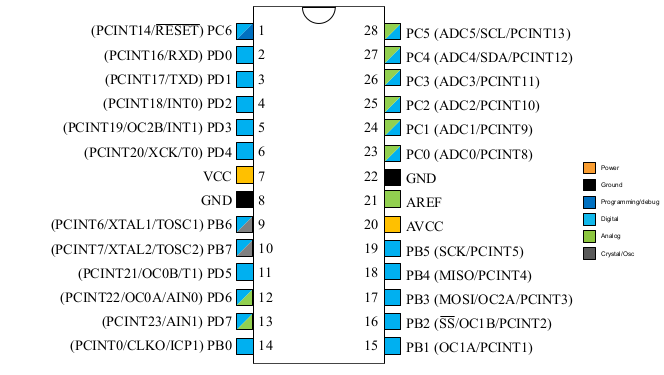
\includegraphics[scale=0.8]{./images/pines.png} 
\caption{Diagrama de pines ATmega328P \cite{atmega328P}.}
\label{f1}
\end{figure}

\begin{figure}[H]
\centering
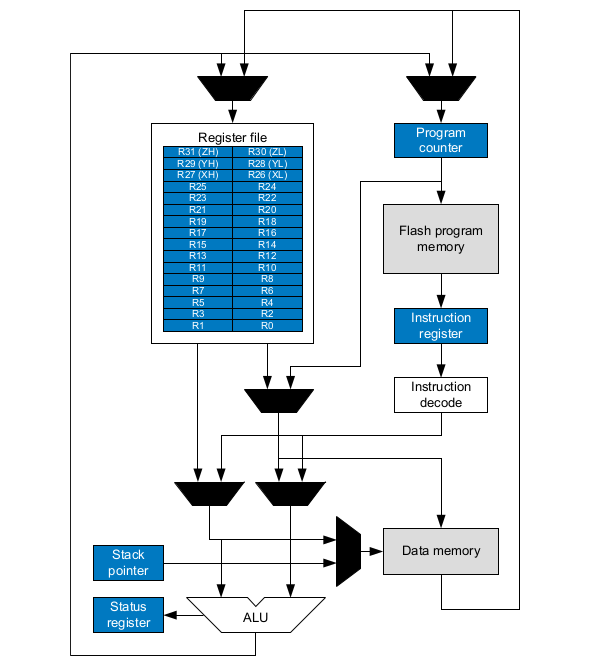
\includegraphics[scale=0.8]{./images/bloques.png} 
\caption{Diagrama de bloques ATmega328P \cite{atmega328P}.  }
\label{f1}
\end{figure}